\newpage
\section{Pangenome de gènes}

\subsection{Généralités et concepts}

Les outils basés sur des pangénomes de gènes, aussi appelés \textit{Presence-absence variation pangenome}s (en anglais, PAV), représentent une grande part des outils de pangénomique procaryote. Le génome des procaryotes étant majoritairement codant, et ce type de pangénome étant plus facile à manipuler et à interpréter, de nombreuses études utilisent les gènes comme unité pour construire les pangénomes. Pour construire ces pangénomes, on commence par regrouper les gènes en familles de gènes, puis on partitionne\footnote{N.B : Dans la suite, pour ne pas faire de confusion entre le partitionnement des familles et le partitionnement des gènes en famille de gènes, nous utiliserons le terme clustering pour parler de la construction des familles de gènes.} les familles en fonction de leur présence dans les génomes (\textit{core}, \textit{accessory}\dots).

% \newpage
\paragraph{Construction des familles de gènes}

La construction des familles de gènes consiste à appliquer une méthode de clustering des gènes par similarité, que nous avons vue en \autoref{sec:clustering}. Le choix de la méthode et des seuils appliqués dans le clustering auront un impact important sur le pangénome. L'outil de clustering influencera aussi l'interprétation. Tout d’abord, les outils d’analyse peuvent s’appuyer sur différents niveaux d’information, tels que la séquence nucléotidique ou protéique, la structure tridimensionnelle des protéines ou encore la fonction biologique associée. Le choix de cette base de comparaison influence de manière déterminante le calcul de la similarité, et par extension, l’inférence du caractère homologue. De plus, en utilisant un outil qui construit des clusters (et donc des familles) d'orthologues, comme orthoMCL \cite{li_orthomcl_2003} ou la base de données COG (cluster of orthologous genes), on retrouvera dans la même famille les gènes ayant suivi les mêmes événements de spéciation. Si l'outil permet de différencier les paralogues des orthologues comme InParanoïd \cite{remm_automatic_2001}, il y aura plus de familles que si on prenait en compte uniquement l'homologie. Le choix de la méthode de clustering est donc essentiel.

\paragraph{Partitionnement du pangénome}

Une fois que les génomes ont été annotés et les familles de gènes construites, les familles de gènes sont partitionnées en fonction de leur présence/absence dans les génomes. Dans les premières analyses, les familles étaient séparées en 2 parties (\autoref{fig:pangenome2}), les familles qui sont présentes dans tous les génomes sont dites "c\oe ur" (\textit{core} en anglais) et les autres sont dites "accessoire" (\textit{accessory} ou \textit{dispensable} en anglais). Cette dichotomie en \textit{core genome} et \textit{accessory genome} est liée au caractère essentiel ou non des fonctions codées par les gènes. Les familles "\textit{core}" sont impliquées dans les processus cellulaires vitaux, ce qui crée une forte pression de sélection de leurs gènes et une forte conservation dans l'ensemble des génomes. À l'inverse, les familles accessoires sont plutôt liées à des adaptations à l'environnement, à un mode de vie\dots. Leurs gènes sont donc moins soumis à la pression de sélection et donc moins conservés dans les génomes.

\begin{figure}[htbp]
    \centering
    \subfloat[Pangénome bipartie]{
        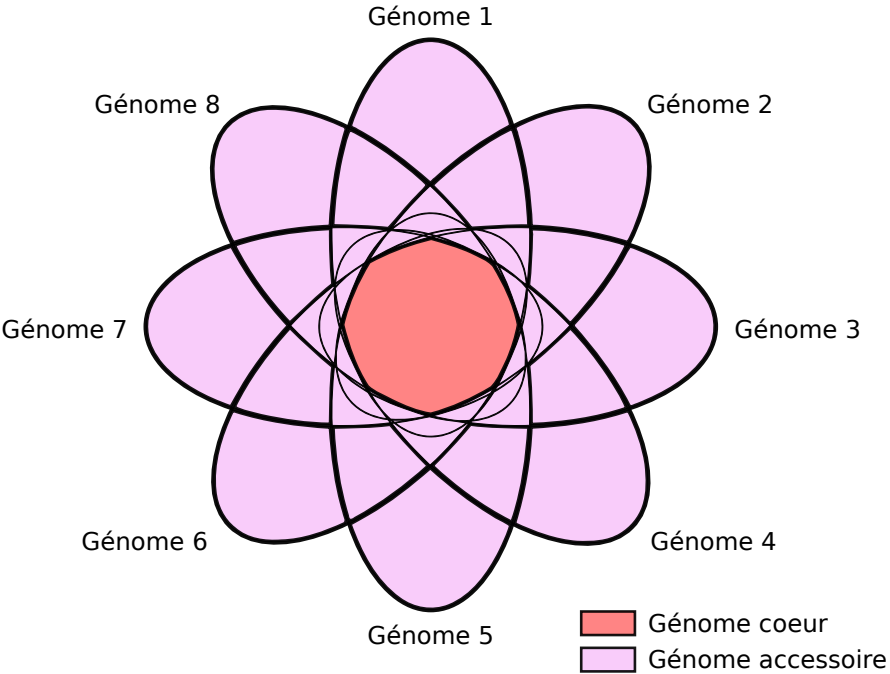
\includegraphics[width=0.48\linewidth]{images/pangenome2.png}
        \label{fig:pangenome2}
    }
    \hfill
    \subfloat[Pangénome tripartie]{
        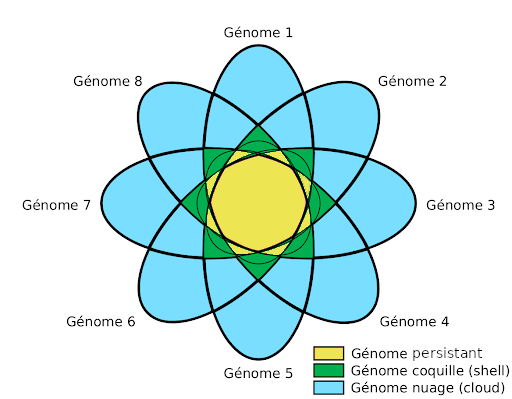
\includegraphics[width=0.48\linewidth]{images/pangenome3.png}
        \label{fig:pangenome3}
    }
    \caption[Partitionnement des pangénomes.]{\textbf{Partitionnement des pangénomes.} Extrait et adapté de \cite{gautreau_conceptualisation_2020}}
    \label{fig:pangenomeVenn}
\end{figure}

\newpage
Ce partitionnement du pangénome en 2 parties, bien que largement utilisé, est une vision très limitée de la distribution des gènes dans les génomes, qui peut amener à des erreurs d'interprétation. Il faut d'abord prendre en compte que même si le nombre de génomes disponibles est de plus en plus conséquent, il n'est toutefois pas possible d'avoir l'ensemble des génomes d'une espèce (cf. \autoref{sec:croissance_pan}), ce qui implique qu'il est plus que probable que des gènes soient identifiés comme accessoires alors qu'ils sont \textit{core} et inversement. 
De plus, les techniques de séquençage et les outils bioinformatiques ne sont pas infaillibles, et donc une erreur d'assemblage, d'annotation, de regroupement en familles, ou encore l'utilisation de génomes partiels, peut entraîner le mauvais classement d'une famille. Pour répondre à ce problème, Lapierre et Gogarten \cite{lapierre_estimating_2009} suggèrent de définir un c\oe ur relâché (\textit{soft-core} en anglais), qui contient les familles présentes dans 95 \% des génomes\footnote{ce pourcentage peut varier en fonction des études.}. Une autre proposition, de Snippen \textit{et al.} \cite{snipen_microbial_2009} raffinant un modèle proposé par Hogg \textit{et al.} \cite{hogg_characterization_2007}, rendrait le nombre de partitions variable en fonction du contenu du pangénome. Cette dernière proposition permet de ne pas utiliser de seuil fixe pour partitionner les familles.
En parallèle, Koonin \textit{et al.}, dans une analyse de l'ensemble des génomes procaryotes disponibles en 2008 \cite{koonin_genomics_2008}, et Makarova \textit{et al.}, en étudiant l'ensemble des génomes d'archées disponibles en 2007 \cite{makarova_clusters_2007}, proposent une vision tripartie du pangénome (\autoref{fig:pangenome3}). Les 2 articles suivent une méthodologie similaire : après une annotation fonctionnelle des génomes, ils comptabilisent le nombre de génomes associés à chaque fonction (COGs pour Makarova et EggNOGs \cite{jensen_eggnog_2008} pour Koonin). Les résultats obtenus révèlent une distribution en forme de courbe en U, où chaque extrémité correspond à une catégorie spécifique de fonctions, tandis que la base regroupe une autre catégorie distincte. Ils redéfinissent alors le core genome comme l’ensemble des gènes présents dans la quasi-totalité des génomes. Ce \textit{core genome} relâché et flexible (sans seuil) est aussi appelé \textit{soft-core genome}, ou encore \textit{persistent genome}, dans certains articles pour le différencier du \textit{core genome} strict défini en premier. L'\textit{accessory genome} sera lui divisé en 2, le \textit{cloud genome} correspondant aux gènes partagés par un faible nombre de génomes, et le \textit{shell genome} correspondant aux gènes ayant une fréquence intermédiaire dans les génomes. Ces différents partitionnements, qui ne sont pas incompatibles, sont de plus en plus utilisés, dû au nombre croissant de génomes disponibles. 

\paragraph{Modélisation et représentation des pangénomes de gènes}

Pour représenter les pangénomes de gènes, il est possible d'utiliser une matrice de présence/absence des gènes (\autoref{fig:panType}B). Cette représentation permet de rapidement identifier le \textit{core genome} ou de trouver les gènes spécifiques à un génome d'intérêt par exemple. Une seconde représentation est celle du diagramme de Venn (\autoref{fig:pangenomeVenn}). À partir du diagramme, on peut rapidement avoir une idée de la proportion de chaque partie, et aussi de la "croissance" du pangénome. Ces 2 représentations ont l'intérêt d'être simples à calculer et à interpréter, néanmoins, lorsque le nombre de génomes devient trop important, il n'est plus possible de les visualiser correctement. De plus, elles se focalisent exclusivement sur le contenu en gènes des génomes, sans fournir d’informations sur leur arrangement ou leur structure organisationnelle.

Afin d’intégrer l’organisation des gènes en plus de leur simple présence, une approche alternative repose sur une représentation où les gènes et leurs relations sont modélisés sous forme de graphe. Dans ce graphe, les familles de gènes constituent les n\oe uds et les relations de voisinage entre les gènes correspondent aux arêtes. Sur la \autoref{fig:graphPanFam}, on peut voir que dans cette représentation, plus les familles ont des gènes voisins, plus le poids de l'arête (épaisseur) augmente. Le graphe de pangénome permet alors d'identifier des structures ou des chemins de familles conservées, ou à l'inverse des régions fortement variables.

\begin{figure}[htbp]
    \centering
    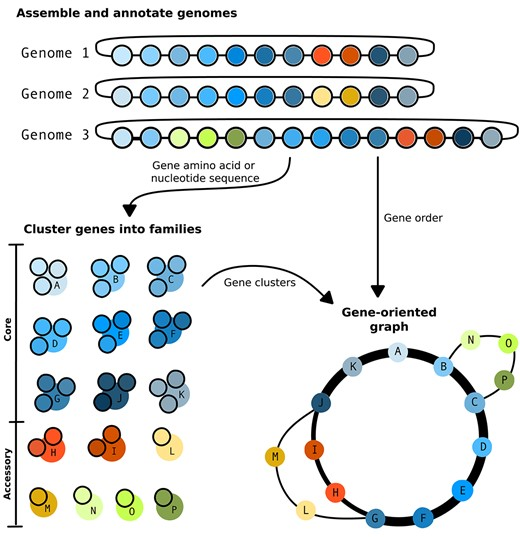
\includegraphics[width=0.8\linewidth]{images/graphePanFam.jpeg}
    \caption[Représentation d'un pangénome de gènes sous forme de graphe]{\textbf{Représentation d'un pangénome de gènes sous forme de graphe.} Extrait de \cite{matthews_gentle_2024}}
    \label{fig:graphPanFam}
\end{figure}

\subsection{Méthodes et outils de pangénome de gènes}

Le premier outil dédié à la construction de pangénomes de famille de gènes est Edgar \cite{blom_edgar_2009}. Disponible en ligne, ce n'est pas un outil à proprement parler, mais plutôt une ressource de résultats d'analyse de pangénome. Dans sa méthode, Edgar clusterise les gènes en familles d'orthologues, en utilisant le BBH\footnote{\textit{Bidirectional Best Hit}}. Les génomes étant relativement proches dans les analyses, les paralogues récents pourraient être regroupés avec des orthologues. Les familles sont donc raffinées en utilisant un système de score pour valider les BBH. Dans sa version actuelle, l'outil permet d'identifier le \textit{core genome} et l'\textit{accessory genome}, rechercher des synténies conservées, de construire des arbres phylogénétiques, ou encore d'annoter fonctionnellement les gènes à partir de bases de données de référence.

Le premier outil permettant la construction de pangénome en ligne de commande est PGAP \cite{zhao_pgap_2012}. Le premier intérêt de PGAP, est qu'il permet à l'utilisateur de construire un pangénome avec ses propres génomes. PGAP construit lui aussi des familles d'orthologues. À partir de ces familles, il propose différentes analyses, comme la courbe de raréfaction, le profil du pangénome\footnote{Le nombre de gènes (y) présents dans x génomes.}, l'identification du \textit{core genome}, l'analyse de variants. Une interface PGAP-X \cite{zhao_pgap-x_2018} rend l'outil plus accessible et améliore la visualisation des résultats.

PanOCT \cite{fouts_panoct_2012} est un autre outil disponible en ligne de commande. Il propose aussi un clustering en famille orthologues, similaire à EDGAR, mais améliore l'algorithme en ajoutant l'information de contexte conservé (\textit{Conserved Gene Neighborhood}, CGN). Les gènes orthologues ont tendance à conserver leur organisation génomique dans les espèces proches contrairement aux espèces éloignées et aux gènes paralogues \cite{huynen_measuring_1998,rocha_organization_2008}. En combinant le BBH et le CGN, les familles de gènes orthologues sont de meilleure qualité. L'outil PanACEA \cite{clarke_panacea_2018} récupère les familles de PanOCT et permet de visualiser le pangénome, mais aussi de l'annoter, notamment avec des informations liées à l'antibiorésistance. 

PanFunPro \cite{lukjancenko_panfunpro_2013}, propose une méthode originale pour construire des familles de gènes homologues, en se basant sur l'annotation fonctionnelle des protéines. Pour annoter les protéines, il utilise des profils HMM de différentes bases de données de domaines protéiques. En définissant l’homologie selon la fonction plutôt que la séquence, cette approche propose un cadre d’analyse alternatif, privilégiant les similarités fonctionnelles des protéines et offrant ainsi une vision complémentaire aux méthodes traditionnelles.

Roary \cite{page_roary_2015} est l'outil de pangénomique certainement le plus utilisé et le plus célèbre. Sa popularité vient de sa capacité à générer des pangénomes de façon rapide en demandant peu de ressources par rapport à ses concurrents de l'époque. Pour ça, il utilise un algorithme CD-Hit pour grouper les séquences proches avant d'aligner les séquences représentantes entre elles avec BLASTP. Les familles sont construites avec l'algorithme MCL et raffinées en utilisant les informations de colocalisation. Roary est aussi un des premiers programmes à représenter les pangénomes de gènes sous forme d'un graphe dans lequel les n\oe uds sont les gènes et les arêtes représentent une relation de voisinage dans les génomes.

\newpage
D'autres outils vont reprendre ce modèle de graphe de gènes, comme Panaroo \cite{tonkin-hill_producing_2020}. À partir du graphe, il corrige les erreurs d'annotation et d'assemblage. Il dispose également de plusieurs modules d'analyse : GWAS, SV, phylogénie et visualisation du pangénome. Panaroo est un outil performant, mais demande des ressources de calcul relativement importantes et une expertise bioinformatique plus importante que d'autres outils. De plus, en nettoyant le graphe, il est possible qu'il élimine des évènements évolutifs récents, et donc ne pas être adapté à des taxons dans lesquels les taux de HGT sont élevés par exemple. Panakeia \cite{beier_panakeia_2022} est un outil reposant aussi sur un modèle de graphe de pangénome, mais propose une analyse plus "universelle". L'outil propose entre autres l'identification de chemins particuliers dans le graphe, correspondant à des structures biologiques, comme les îlots génomiques.

Les outils présentés jusqu'ici, bien que non limités théoriquement, sont généralement appliqués à la construction de pangénomes au niveau de l'espèce. Des méthodes, comme RIBAP \cite{lamkiewicz_ribap_2024}, proposent de construire des pangénomes au niveau du genre. RIBAP construit un pangénome en utilisant ROARY à 95 \% d'identité. En parallèle, il utilise MMSeqs2 pour aligner l'ensemble des gènes. Le résultat de l'alignement est ensuite utilisé pour raffiner les familles pour construire des familles homologues au niveau du genre. De cette manière, la partie de \textit{core genome} est plus importante. Avec ce nouveau partitionnement, RIBAP propose de construire un arbre phylogénétique des souches présentes dans le pangénome. 

L'utilisation de pangénomes de gènes est bien adaptée à la génomique comparée des procaryotes. Leur simplicité de calcul et d'interprétation les rend accessibles pour tous les utilisateurs. Néanmoins, cette simplicité est liée à une vision gène centrée, qui ne prend pas en compte les régions non codantes. Des outils, comme Piggy \cite{thorpe_piggy_2018}, permettent de pallier ce problème en proposant une analyse complémentaire à un pangénome de gène généré par Roary. Ainsi, la complémentarité des outils permet d'avoir une étude plus complète. 

En 2020, PPanGGOLiN \cite{gautreau_ppanggolin_2020} introduit une stratégie de partitionnement, s’appuyant sur un algorithme de \textit{machine learning} pour classifier les gènes du pangenome. Cette approche repose sur une analyse des relations de voisinage et du clustering, éliminant ainsi la nécessité de fixer des seuils stricts. Par conséquent, PPanGGOLiN permet d’identifier de manière dynamique les trois composantes du pangenome — \textit{persistent genome}, \textit{shell genome} et \textit{cloud genome} — sans présupposer de leur répartition.

\subsection{Analyses à partir de pangénomes de gènes}

Les pangénomes de gènes sont utilisés pour mener des études de phylogénomique. En 2020, Gaba \textit{et al.} \cite{gaba_pan-genome_2020} s'intéressent aux archées de la classe des Halobacteria, des archées extrêmement halophiles\footnote{Capable de vivre dans des milieux à haute concentration en sel}. Ils vont construire un pangénome à l'aide de l'outil GET\textunderscore HOMOLOGUE \cite{contreras-moreira_get_homologues_2013}, un outil similaire à EDGAR. À partir de ce pangénome, ils ont pu identifier les gènes \textit{core} des gènes \textit{accessory}. Sur la base de ce partitionnement, ils ont pu mettre en évidence un fort taux de transferts horizontaux au sein de la classe des Halobacteria. Ils ont alors construit une phylogénie basée sur le pangénome et sa partition, mettant en évidence une évolution étroite entre l'ordre des Natrialbales et celui des Halobacteriales, suggérant alors l'existence d'un superordre les regroupant. Plusieurs méthodes permettent d’ailleurs d'identifier les régions où les transferts horizontaux de gènes se produisent préférentiellement. Parmi elles, la méthode panRGP\cite{bazin_panrgp_2020} permet de détecter les régions de plasticité génomique (RGP), \textit{i.e.} des segments du génome échangés entre différentes souches par transfert horizontal ou perdus de manière différentielle selon les lignées. Cette approche repose sur l’analyse du graphe de pangénome et de sa partition pour identifier les régions variables. Elle permet également d’identifier des spots, en repérant les familles de gènes persistantes flanquant les RGP. Une autre méthode, panModule\cite{bazin_panmodule_2021}, vise quant à elle à détecter des groupes de familles de gènes variables dans le pangénome, qui sont organisés en blocs de synténie au sein des génomes. Ces deux méthodes sont intégrées à la suite logicielle PPanGGOLiN et exploitent le graphe de pangénome généré par cette dernière.

Dans les exemples cités, les études étaient centrées sur des groupes taxonomiques et donc les génomes appartenaient au même taxon. Pourtant, comme nous l'avons déjà vu, l'étude d'environnements et les données métagénomiques sont étroitement liées aux études pangénomiques. Vera-Ponce de León \textit{et al.} \cite{vera-ponce_de_leon_genomic_2024}, produisent un atlas génomique du microbiote des saumons. Pour caractériser les espèces présentes et construire le pangénome, ils utilisent l'outil mOTUpan \cite{buck_motupan_2022}. mOTUpan permet de clusteriser les métagénomes à un fort niveau d'identité (95 \%), définissant ainsi des unités taxonomiques opérationnelles métagénomiques (mOTUs, \textit{metagenomic Operational Taxonomic Unit} en anglais). Chaque mOTU peut être associé à une espèce (ou un taxon) et donc permettre de séparer les gènes appartenant à la même espèce dans une même mOTU. L'intérêt de mOTUpan est qu'il utilise un modèle bayésien pour estimer le génome \textit{core} et le génome accessoire. Ce modèle prend en compte la complétion (souvent faible) des métagénomes et améliore la qualité du partitionnement sur ces données. À partir du pangénome, les auteurs ont pu identifier 14 ordres bactériens différents, représentant 35 genres distincts, ils ont également identifié 29 nouvelles espèces encore non répertoriées.

Les méthodes de machine learning peuvent aussi être utilisées pour analyser les pangénomes. Dans leur article, Kavvas \textit{et al.} \cite{kavvas_machine_2018} proposent d'utiliser des méthodes de machine learning pour identifier des gènes de résistance aux antibiotiques dans 1 595 souches de \textit{Mycobacterium tuberculosis}. Le pangénome est construit à partir de familles homologues, et les gènes connus pour être des gènes de résistance aux antibiotiques sont annotés. En utilisant des méthodes de machine learning (SVM, MI, ANOVA\dots), les auteurs ont pu identifier 24 nouveaux gènes de résistance, de plus le signal de certains gènes déjà connus est plus fort que mesuré précédemment. Les auteurs ont poursuivi en analysant la structure des nouveaux gènes et de leurs protéines, ainsi qu'en menant une étude géographique de la répartition des gènes pour établir des liens entre population hôte et résistance. Il faut néanmoins rappeler une nouvelle fois que la découverte de ces nouveaux gènes doit être vérifiée et que leur identification n'est possible que sur la base d'une base de données de gènes connus.

\begin{table}[htbp]
  \centering
  \footnotesize
  \begin{tabular}{|p{.2\textwidth}|p{.38\textwidth}|p{.35\textwidth}|}
    \hline
    Nom & Méthode & Référence \\
    \hline
    EDGAR & matrice présence/abscence & \cite{blom_edgar_2009}\\
    \hline
    PGAP & matrice présence/abscence & \cite{zhao_pgap_2012}\\
    \hline
    PanOCT & Clustering d'orthologue & \cite{fouts_panoct_2012}\\
    \hline
    GET\textunderscore HOMOLOGUES & Clustering d'orthologue & \cite{contreras-moreira_get_homologues_2013} \\
    \hline
    PanACEA & Visualisation & \cite{clarke_panacea_2018}\\
    \hline
    PanFunPro & Familles de profil fonctionnelle & \cite{lukjancenko_panfunpro_2013}\\
    \hline
    Roary & Graphe de famille de gène & \cite{page_roary_2015}\\
    \hline
    Piggy & Analyse région intergénique & \cite{thorpe_piggy_2018}\\
    \hline
    Ptolemy & Graphe de famille de gène & \cite{thorpe_piggy_2018}\\
    \hline
    PIRATE & Graphe de famille de gène & \cite{bayliss_pirate_2019}\\
    \hline
    Panaroo & Graphe de famille de gène & \cite{tonkin-hill_producing_2020}\\
    \hline
    PPanGGOLiN & Graphe de famille de gène & \cite{gautreau_ppanggolin_2020}\\
    \hline
    PanACoTA & Graphe \& Phylogénie & \cite{perrin_panacota_2021} \\
    \hline
    Panakeia & Graphe de famille de gène & \cite{beier_panakeia_2022}\\
    \hline
    PanPhlAn & Graphe de données métagénomique & \cite{scholz_strain-level_2016}\\
    \hline
    MSPminer & Graphe de données métagénomique & \cite{plaza_onate_mspminer_2019}\\
    \hline
    mOTUpan & Graphe de données métagénomique & \cite{buck_motupan_2022}\\
    \hline
    Pan-Tetris & Visualisation & \cite{hennig_pan-tetris_2015}\\
    \hline
    PanViz & Visualisation & \cite{pedersen_panviz_2017}\\
    \hline
    Panache & Visualisation & \cite{durant_panache_2021}\\
    \hline
    
  \end{tabular}
  \caption[Outils de pangénomique basés sur les familles de gènes]{\textbf{Liste non exhaustive d'outils de pangénomique basés sur les familles de gènes}}
  \label{tab:pangenomicToolsFam}
\end{table}